\usetikzlibrary{matrix,patterns,arrows.meta,decorations.pathreplacing,shapes.misc,fit}

\begin{frame}[fragile,label=redirectExample]{shell redirection}
\begin{itemize}
\item \verb|./my_program ... < input.txt|:
    \begin{itemize}
    \item run \verb|./my_program ...| but use \verb|input.txt| as input
    \item like we copied and pasted the file into the terminal
    \end{itemize}
\vspace{.5cm}
\item \verb|echo foo > output.txt|:
    \begin{itemize}
    \item runs \verb|echo foo|, sends output to \verb|output.txt|
    \item like we copied and pasted the output into that file
    \item (as it was written)
    \end{itemize}
\end{itemize}
\end{frame}

\begin{frame}[fragile,label=forkTrick]{fork copies file pointer list}
\begin{tikzpicture}
\tikzset{
    >=Latex,
    pcb/.style={
        tight matrix,
        column 1/.style={nodes={draw,thin,text width=2.5cm,font=\small,minimum height=0.45cm}},
        column 2/.style={nodes={draw,thin,text width=4.75cm,font=\fontsize{9}{10}\tt\selectfont,minimum height=0.45cm}},
    },
    page/.style={
        draw,thick,
        pattern=north west lines,
        minimum width=2cm,
        node contents={~},
    },
    pointer/.style={
        draw,very thick,-Latex,
    },
    pointer light/.style={
        draw,thick,-Latex,
    },
    tall/.style={
        minimum height=0.85cm
    },
    taller/.style={
        minimum height=1.2cm
    },
    one pt/.style={
        fill=blue!40,
    },
    one pt line/.style={
        draw=blue!80!black,
        alt=<2->{opacity=0.0},
    },
    one memory/.style={
        fill=green!40,
    },
    one memory line/.style={
        draw=green!80!black,
        alt=<2->{opacity=0.0},
    },
    two pt/.style={
        fill=orange!40,
    },
    two pt line/.style={
        draw=orange!80!black,
        alt=<2->{opacity=0.0},
    },
    two memory/.style={
        fill=violet!40,
    },
    two memory line/.style={
        draw=violet!80!black,
        alt=<2->{opacity=0.0},
    },
    fork line/.style={
        draw=black!30,line width=2mm,-{Latex[length=6mm]}
    },
    marked/.style={draw=red,ultra thick},
}
\matrix[pcb,label={[font=\small]north:parent process control block}] (proc one) {
    |[tall]| user regs \&
    |[tall]|
    {eax=\sout<1->{42}\only<1->{\textit{\myemph<0>{child (new) pid}}}, \\ ecx=133,} \ldots \\
    page table \& |[one pt]| ~ \\
    |[taller]| open files \& |[taller,marked,alias=old files]| {fd 0: \ldots \\ fd 1: \ldots \\ \ldots } \\
    \ldots \& \ldots \\
};
\newcommand{\halfvthick}{.2mm}
\node[draw,very thick,pattern=north west lines,minimum width=1.5cm,minimum height=3cm,anchor=north west,
    label={north:memory}] (memory) at ([xshift=3cm,yshift=0cm]proc one.north east) {};
\draw[pointer,one pt line] (proc one-2-2.east) -- ++(1cm,0cm) |- ([yshift=-1.3cm]memory.north west);
\foreach \y in {-1.3cm} {
    \draw[very thick,one pt] ([yshift=\y,xshift=\halfvthick]memory.north west) rectangle ++ (1.5cm,-1mm);
}
\coordinate (one pt loc) at ([yshift=-1.35cm,xshift=\halfvthick]memory.north west);
\draw[pointer light,one memory line] ([yshift=-.1mm]one pt loc) -- ++(-.25cm,0cm) |- ([yshift=-0.1cm]memory.north west);
\draw[pointer light,one memory line] ([yshift=-.2mm]one pt loc) -- ++(-.35cm,0cm) |- ([yshift=-0.6cm]memory.north west);
\draw[pointer light,one memory line] ([yshift=.3mm]one pt loc) -- ++(-.45cm,0cm) |- ([yshift=-0.7cm]memory.north west);
\foreach \y in {-0.5cm,-0.7cm,-0.8mm} {
    \draw[very thick,one memory] ([yshift=\y,xshift=\halfvthick]memory.north west) rectangle ++ (1.5cm,-1mm);
}
\matrix[pcb,anchor=north west,label={[font=\small]north:child process control block}] (proc two) at ([yshift=-1cm]proc one.south west) {
    |[tall]| user regs \&
    |[tall]|
    {eax=\sout<1->{42}\only<1->{\myemph<0>{0}}, \\ ecx=133, \ldots} \\
    pagetable \& |[two pt]| ~ \\
    |[taller]| open files \& |[taller,marked,alias=new files]| {fd 0: \ldots \\ fd 1: \ldots \\ \ldots } \\
    \ldots \& \ldots \\
};
\draw[fork line] ([xshift=-0.25cm]proc one.west) -- ++(-1cm,0cm) |- ([xshift=-0.25cm]proc two.west)
    node[pos=0.25,right] {copy};
\draw[pointer,two pt line] (proc two-2-2.east) -- ++(1cm,0cm) |- ([yshift=-2.3cm]memory.north west);
\foreach \y in {-2.3cm} {
    \draw[very thick,two pt] ([yshift=\y,xshift=\halfvthick]memory.north west) rectangle ++ (1.5cm,-1mm);
}
\coordinate (two pt loc) at ([yshift=-2.35cm,xshift=\halfvthick]memory.north west);
\draw[pointer light,two memory line] ([yshift=-.1mm]two pt loc) -- ++(-.75cm,0cm) |- ([yshift=-2.4cm]memory.north west);
\draw[pointer light,two memory line] ([yshift=-.2mm]two pt loc) -- ++(-.85cm,0cm) |- ([yshift=-2.6cm]memory.north west);
\draw[pointer light,two memory line] ([yshift=-.3mm]two pt loc) -- ++(-.95cm,0cm) |- ([yshift=-2.7cm]memory.north west);
\foreach \y in {-2.4cm,-2.6cm,-2.7cm} {
    \draw[very thick,two memory] ([yshift=\y,xshift=\halfvthick]memory.north west) rectangle ++ (1.5cm,-1mm);
}
\draw[fork line] ([yshift=-0.9cm,xshift=.5cm]memory.north east) coordinate (one memory)-- ++(1.2cm, 0cm) |- ([yshift=-2.6cm,xshift=.5cm]memory.north east) coordinate (two memory)
    node[pos=0.25,left] {copy};
\draw[ultra thick,decorate,decoration={brace,mirror}] ([xshift=-.25cm,yshift=-8mm]one memory) -- ([xshift=-.25cm,yshift=8mm]one memory);
\draw[ultra thick,decorate,decoration={brace,mirror}] ([xshift=-.25cm,yshift=-4mm]two memory) -- ([xshift=-.25cm,yshift=4mm]two memory);
\begin{visibleenv}<2->
\node[draw, very thick,anchor=north west,font=\small,align=left] (fd0) at ([yshift=-1cm,xshift=-2.5cm]memory.south) {
    open file description (stdin)
};
\node[draw, very thick,anchor=north west,font=\small,align=left] (fd1) at ([yshift=-1mm]fd0.south west) {
    open file description (stdout)
};
\draw[violet,->,ultra thick] ([xshift=1.5cm,yshift=-.25cm]old files.north west) -| ([xshift=-1cm]fd0.west) -- (fd0.west);
\draw[violet,->,ultra thick] ([xshift=1.5cm,yshift=-.25cm]new files.north west) -| ([xshift=-1cm]fd0.west) -- (fd0.west);
\draw[blue,->,ultra thick] ([xshift=1.5cm,yshift=-.55cm]old files.north west) -| ([xshift=-.75cm]fd1.west) -- (fd1.west);
\end{visibleenv}
\begin{visibleenv}<2>
\draw[blue,->,ultra thick] ([xshift=1.5cm,yshift=-.55cm]new files.north west) -| ([xshift=-.75cm]fd1.west) -- (fd1.west);
\end{visibleenv}
\begin{visibleenv}<3->
    \draw[blue,->,opacity=0.5,ultra thick] ([xshift=1.5cm,yshift=-.55cm]new files.north west) -| ([xshift=-.75cm]fd1.west) -- (fd1.west);
\node[draw,dotted,red,fill=red!5,ultra thick,anchor=north west,font=\small,align=left] (fd2) at ([yshift=-1mm]fd1.south west) {
    redirected-to stdout? \\
    (set after fork, before exec)
};
\draw[red,dotted,->,line width=1.2mm] ([xshift=1.5cm,yshift=-.55cm]new files.north west) -| ([xshift=-.75cm]fd2.west) -- (fd2.west);
\end{visibleenv}
\end{tikzpicture}
\end{frame}

\begin{frame}[fragile,label=typicalPatternRedirect]{typical pattern with redirection}
\newcommand{\maincode}{
            pid = fork(); \\
            if (pid == 0) \{ \\
            \hspace{.5cm} open new files; \\
            \hspace{.5cm} exec\ldots(\ldots); \\
            \hspace{.5cm} \ldots \\
            \} else if (pid > 0) \{ \\
            \hspace{.5cm} waitpid(pid,\ldots); \\
            \hspace{.5cm} \ldots \\
            \} \\
            \ldots
        }
\newcommand{\maincodeWait}{
            pid = fork(); \\
            if (pid == 0) \{ \\
            \hspace{.5cm} open new files; \\
            \hspace{.5cm} exec\ldots(\ldots); \\
            \hspace{.5cm} \ldots \\
            \} else if (pid > 0) \{ \\
            \hspace{.5cm} \myemph{waitpid(pid,\ldots)}; \\
            \hspace{.5cm} \ldots \\
            \} \\
            \ldots
        }
\newcommand{\maincodeFork}{
            pid = \myemph{fork()}; \\
            if (pid == 0) \{ \\
            \hspace{.5cm} open new files; \\
            \hspace{.5cm} exec\ldots(\ldots); \\
            \hspace{.5cm} \ldots \\
            \} else if (pid > 0) \{ \\
            \hspace{.5cm} waitpid(pid,\ldots); \\
            \hspace{.5cm} \ldots \\
            \} \\
            \ldots
        }
\newcommand{\maincodeOpenNew}{
            pid = fork(); \\
            if (pid == 0) \{ \\
            \hspace{.5cm} \myemph{open new files}; \\
            \hspace{.5cm} exec\ldots(\ldots); \\
            \hspace{.5cm} \ldots \\
            \} else if (pid > 0) \{ \\
            \hspace{.5cm} waitpid(pid,\ldots); \\
            \hspace{.5cm} \ldots \\
            \} \\
            \ldots
}
\newcommand{\altcode}{
            main() \{ \\
            \hspace{.5cm} \ldots \\
            \}
}
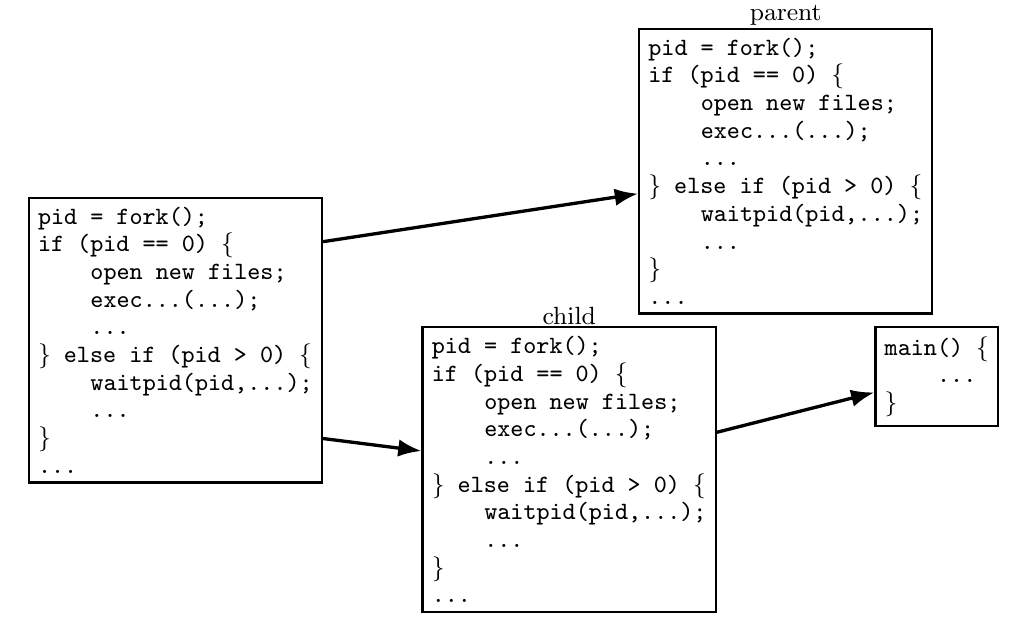
\begin{tikzpicture}
\tikzset{
    code box/.style={draw,thick,font=\tt\fontsize{9}{10}\selectfont,align=left},
    with the code/.style={
        code box,
    },
    with the other code/.style={
        code box,
    }
}
\node[with the code] (start) {\maincodeFork};
\node[with the code,anchor=south west,
      label={[font=\small,label distance=-1mm,overlay]north:parent}] (parent first) at ([xshift=4cm,yshift=-1.5cm]start.north east) {\maincodeWait};
\node[with the code,anchor=north west,
      label={[font=\small,label distance=-1mm]north:child}] (child first) at ([xshift=1.25cm,yshift=2cm]start.south east) {\maincodeOpenNew};
\node[with the other code,anchor=north west] (child second) at ([xshift=2cm]child first.north east) {\altcode};

\begin{scope}[very thick,>=Latex]
\draw[->] ([yshift=1.25cm]start.east) -- (parent first);
\draw[->] ([yshift=-1.25cm]start.east) -- (child first);
\draw[->] (child first) -- (child second);
\end{scope}
\end{tikzpicture}
\end{frame}

\begin{frame}{redirecting with exec}
\begin{itemize}
\item standard output/error/input are files
    \begin{itemize}
    \item (C stdout/stderr/stdin; C++ cout/cerr/cin)
    \end{itemize}
\vspace{.5cm}
\item (probably after forking) open files to redirect
\item \ldots and make them be standard output/error/input
    \begin{itemize}
    \item using \texttt{dup2()} library call
    \end{itemize}
\item then exec, preserving new standard output/etc.
\end{itemize}
\end{frame}
